\chapter{Transfer Learning}

% Required packages in the preamble:
% \usepackage{graphicx}
% \usepackage{booktabs}
% \usepackage{float}
% \usepackage{subcaption}

\section{Transfer-Learning Approach and Experimental Setup}
\label{sec:transfer_setup}

In addition to the two simple CNN baselines trained from scratch
(Section~\ref{sec:baselines}), a transfer-learning approach was evaluated
using an EfficientNetB0 backbone pretrained on ImageNet. The motivation was
to test whether features learned on a large, general-purpose image dataset
could improve classification performance on a relatively small,
domain-specific chest radiograph dataset, and whether such a model relies on
the same visual cues as the CNN trained from scratch.

The classification head placed on top of the backbone consisted of:

\begin{center}
\begin{tabular}{l}
\toprule
\textbf{Transfer-Learning Head} \\
\midrule
EfficientNetB0 backbone (ImageNet weights) \\
Global Average Pooling \\
Dropout (rate 0.3) \\
Dense layer, 128 units, ReLU \\
Dropout (rate 0.3) \\
Dense layer, 4-class softmax output \\
\bottomrule
\end{tabular}
\end{center}

Training used the same manifest, the same 70/15/15 stratified train,
validation, and test split, and the same random seed (42) as the CNN
baselines, so results are directly comparable to those reported in
Section~\ref{sec:baselines}.

A two-phase training design was used throughout this chapter. In phase 1,
the EfficientNetB0 backbone was kept frozen and only the classification head
was trained. In several experiments (Section~\ref{sec:transfer_finetune}),
a second phase then unfroze the backbone and continued training end-to-end
at a substantially lower learning rate. This design allowed the new head to
first adapt to the pretrained features before any backbone weights were
disturbed, reducing the risk of destructive early updates.

\section{Baseline Transfer Model}
\label{sec:transfer_baseline}

The first transfer-learning experiment kept the EfficientNetB0 backbone
entirely frozen and trained only the classification head, without
augmentation or class weighting. Its test-set performance is presented in
Table~\ref{tab:transfer_baseline_results}.

\begin{table}[H]
\centering
\caption{Test-set performance of the frozen EfficientNetB0 transfer model.}
\label{tab:transfer_baseline_results}
\begin{tabular}{lccc}
\toprule
\textbf{Class} & \textbf{Precision} & \textbf{Recall} & \textbf{F1-score} \\
\midrule
COVID            & 0.943 & 0.903 & 0.923 \\
Lung Opacity     & 0.906 & 0.808 & 0.854 \\
Normal           & 0.869 & 0.946 & 0.906 \\
Viral Pneumonia  & 0.984 & 0.910 & 0.945 \\
\midrule
\textbf{Macro average} & 0.925 & 0.892 & \textbf{0.907} \\
\bottomrule
\end{tabular}
\end{table}

The frozen transfer model achieved a test accuracy of \textbf{89.70\%} and a
macro F1-score of \textbf{90.7\%}. This already exceeds the strongest
simple-CNN baseline (the full-image model at 81.96\% accuracy and 82.7\%
macro F1, Section~\ref{subsec:full_baseline}) by approximately 7.7 accuracy
points and 8.0 macro-F1 points, without any fine-tuning of the pretrained
backbone. This result confirms that ImageNet-derived features transfer
usefully to this chest radiograph classification task, even though the
source and target domains are visually very different.

\section{Optimisation: Augmentation, Class Weighting, and the Generalisation Gap}
\label{sec:transfer_optimisation}

Following the initial baseline, several optimisation experiments were
conducted to evaluate whether standard machine-learning tools for improving
generalisation and handling class imbalance could improve on the frozen
baseline, in line with the project's Step 2 objective of using statistics
and optimisation tools to fully exploit and understand the model's results.

\subsection{Data Augmentation and the Effect of Horizontal Flipping}
\label{subsec:transfer_augmentation}

An augmentation pipeline combining random horizontal flipping and small
random rotations was first applied during training. Chest radiographs are
not perfectly left-right symmetric in a clinically meaningless way, since
heart position and other incidental laterality cues can appear in the
images, so a second variant disabled horizontal flipping and used rotation
only. Table~\ref{tab:transfer_flip_comparison} compares the two variants on
the test split.

\begin{table}[H]
\centering
\caption{Effect of horizontal flipping on the augmented transfer model (test split).}
\label{tab:transfer_flip_comparison}
\resizebox{\textwidth}{!}{%
\begin{tabular}{lcccccc}
\toprule
\textbf{Model} & \textbf{Accuracy} & \textbf{Macro F1} & \textbf{COVID F1} & \textbf{Lung Opacity F1} & \textbf{Normal F1} & \textbf{Viral Pneumonia F1} \\
\midrule
Flip + rotation      & 87.62\% & 0.884 & 0.879 & 0.832 & 0.892 & 0.935 \\
Rotation only        & \textbf{88.38\%} & \textbf{0.896} & 0.883 & \textbf{0.850} & 0.895 & \textbf{0.956} \\
\bottomrule
\end{tabular}%
}
\end{table}

Removing horizontal flipping improved every test-set metric, with the
largest gains on Lung Opacity (+1.85 F1 points) and Viral Pneumonia (+2.07
F1 points). This is consistent with horizontal flipping introducing a mild,
unhelpful distribution shift for this task rather than a useful invariance,
and suggests that flipping should be treated as a tunable hyperparameter
for chest radiographs rather than an unquestioned default.

\subsection{Class Weighting}
\label{subsec:transfer_class_weighting}

A separate experiment applied class weights inversely proportional to class
frequency, without augmentation, to counter the dataset's imbalance between
the majority Normal and Lung Opacity classes and the minority COVID and
Viral Pneumonia classes. The class-weighted model reached \textbf{88.34\%}
test accuracy and \textbf{0.894} macro F1, close to the augmented
variants. Class weighting mainly redistributed performance toward the
minority classes rather than closing the gap between training and test
performance, indicating that it addresses a different problem (class
imbalance) than augmentation (overfitting).

\subsection{Generalisation Gap Across Runs}
\label{subsec:transfer_generalisation_gap}

Table~\ref{tab:transfer_generalisation_gap} reports the gap between train
and test performance for the frozen baseline and its two augmentation
variants, as a simple diagnostic of overfitting.

\begin{table}[H]
\centering
\caption{Train-test generalisation gap for the frozen-backbone transfer models.}
\label{tab:transfer_generalisation_gap}
\resizebox{\textwidth}{!}{%
\begin{tabular}{lccc}
\toprule
\textbf{Model} & \textbf{Test Accuracy} & \textbf{Accuracy Gap} & \textbf{Macro-F1 Gap} \\
\midrule
Frozen baseline (no augmentation) & 89.70\% & 2.77 pts & 2.67 pts \\
Flip + rotation augmentation      & 87.62\% & 2.72 pts & 2.66 pts \\
Rotation-only augmentation        & 88.38\% & \textbf{1.98 pts} & \textbf{1.27 pts} \\
\bottomrule
\end{tabular}%
}
\end{table}

Rotation-only augmentation roughly halves the frozen baseline's
generalisation gap (1.98 versus 2.77 accuracy points, 1.27 versus 2.67
macro-F1 points) for a comparatively small reduction in raw test accuracy.
This represents a genuine optimisation trade-off: a model that generalises
somewhat better within this dataset, at a small cost in headline
performance, although it does not on its own resolve the background-reliance
concerns raised in Section~\ref{sec:transfer_interpretability}.

\section{Advanced Modelling: Fine-Tuning the Backbone}
\label{sec:transfer_finetune}

Following the project's Step 3 objective of advanced modelling using deep
learning, the EfficientNetB0 backbone was unfrozen and fine-tuned end-to-end
after the initial frozen-head phase. Phase 1 trained the head only for 10
epochs; phase 2 then unfroze the entire backbone and continued training for
15 further epochs at a much lower learning rate ($10^{-5}$, versus $10^{-3}$
for the head-only phase), for 25 epochs in total.

Figure~\ref{fig:transfer_finetuned_history} shows the resulting training
history. Validation loss briefly increases at the start of phase 2, a normal
consequence of unfreezing a large pretrained backbone and updating it for
the first time, before decreasing steadily to a final value substantially
lower than at the end of phase 1 (from 0.310 to 0.189), with validation
accuracy rising from 88.9\% to 93.3\% over the fine-tuning phase.

\begin{figure}[H]
    \centering
    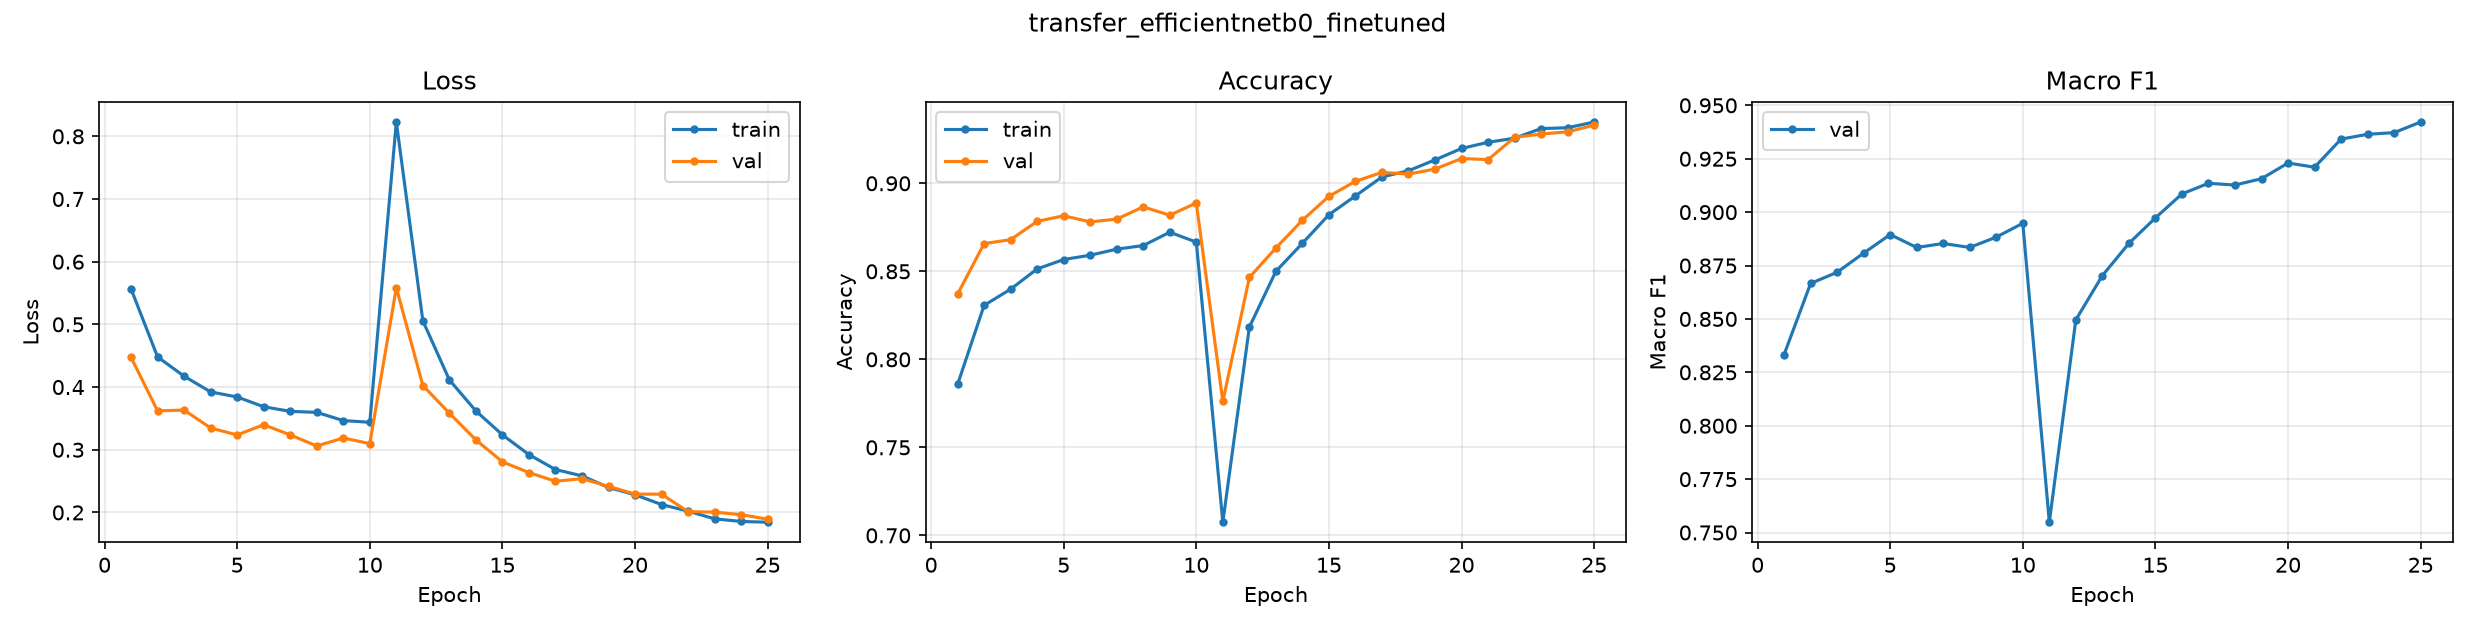
\includegraphics[width=0.8\linewidth]{figures/transfer_finetuned_history.png}
    \caption{Training and validation curves for the fine-tuned EfficientNetB0
    model, showing the frozen-head phase followed by end-to-end fine-tuning.}
    \label{fig:transfer_finetuned_history}
\end{figure}

The fine-tuned model's test-set performance is presented in
Table~\ref{tab:transfer_finetuned_results}.

\begin{table}[H]
\centering
\caption{Test-set performance of the fine-tuned EfficientNetB0 transfer model.}
\label{tab:transfer_finetuned_results}
\begin{tabular}{lccc}
\toprule
\textbf{Class} & \textbf{Precision} & \textbf{Recall} & \textbf{F1-score} \\
\midrule
COVID            & 0.931 & 0.978 & 0.954 \\
Lung Opacity     & 0.958 & 0.814 & 0.880 \\
Normal           & 0.898 & 0.962 & 0.929 \\
Viral Pneumonia  & 0.980 & 0.980 & 0.980 \\
\midrule
\textbf{Macro average} & 0.942 & 0.933 & \textbf{0.936} \\
\bottomrule
\end{tabular}
\end{table}

The fine-tuned model achieved a test accuracy of \textbf{92.36\%} and a
macro F1-score of \textbf{93.6\%}, the strongest result obtained anywhere in
this project. Fine-tuning improved every class relative to the frozen
baseline except Lung Opacity, whose F1-score changed only marginally (0.854
to 0.880), and produced a particularly large gain in COVID recall (90.3\% to
97.8\%). The confusion matrix for this model is shown in
Figure~\ref{fig:transfer_finetuned_confusion}.

\begin{figure}[H]
    \centering
    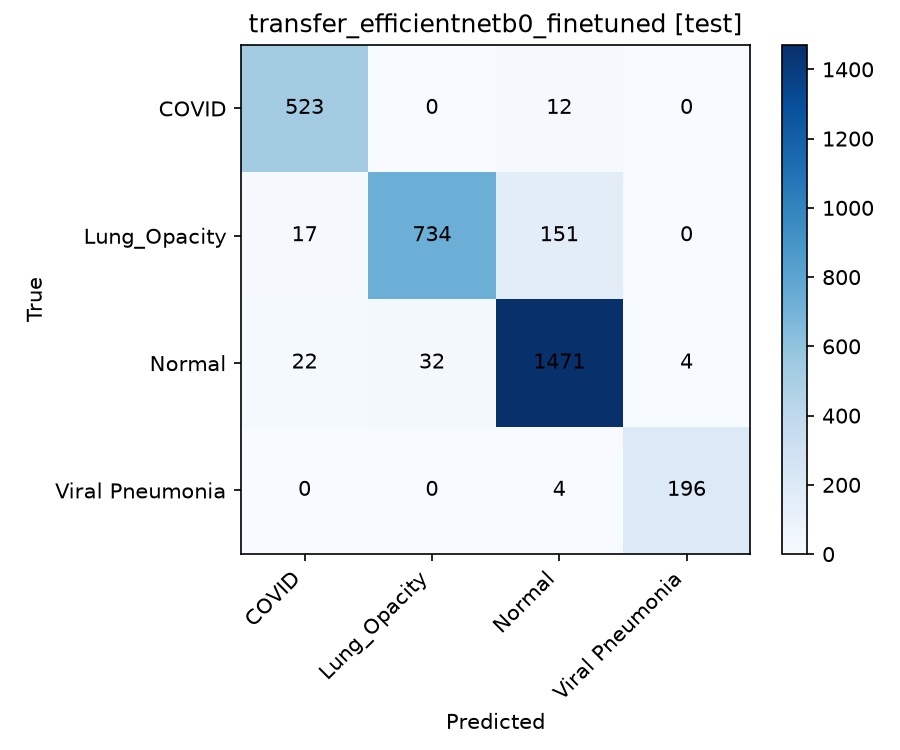
\includegraphics[width=0.55\linewidth]{figures/transfer_finetuned_confusion.png}
    \caption{Test-set confusion matrix for the fine-tuned EfficientNetB0 model.}
    \label{fig:transfer_finetuned_confusion}
\end{figure}

As with the full-image simple-CNN baseline, however, this headline
performance must be interpreted alongside the interpretability analysis
in Section~\ref{sec:transfer_interpretability} before it is read as evidence
of genuinely improved pulmonary diagnosis.

\section{Interpretability: Grad-CAM and the Lung-Focus Causal Analysis}
\label{sec:transfer_interpretability}

Grad-CAM was applied to the transfer-learning models using the same lung
segmentation masks employed for the CNN baselines' interpretability analysis
(Section~\ref{subsec:full_gradcam}). Beyond qualitative visualisation, a
quantitative \emph{lung-focus} metric was computed for every image: the
share of each Grad-CAM heatmap's total activation that falls inside the
segmented lung mask. This is compared against a \emph{chance} level, defined
as the lung mask's own share of the image area, that is, the score a
spatially uninformative model would obtain by construction. A model that
attends to the lungs no more than chance provides no evidence that it is
using pulmonary information specifically.

\subsection{Qualitative and Quantitative Lung Focus of the Frozen Model}
\label{subsec:transfer_lung_focus_baseline}

Figure~\ref{fig:transfer_gradcam_baseline} shows representative Grad-CAM
examples for the frozen transfer model, with the lung boundary overlaid in
green. Heatmaps frequently activate at chest borders, shoulders, or corners
rather than tightly within the lung fields.

\begin{figure}[H]
    \centering
    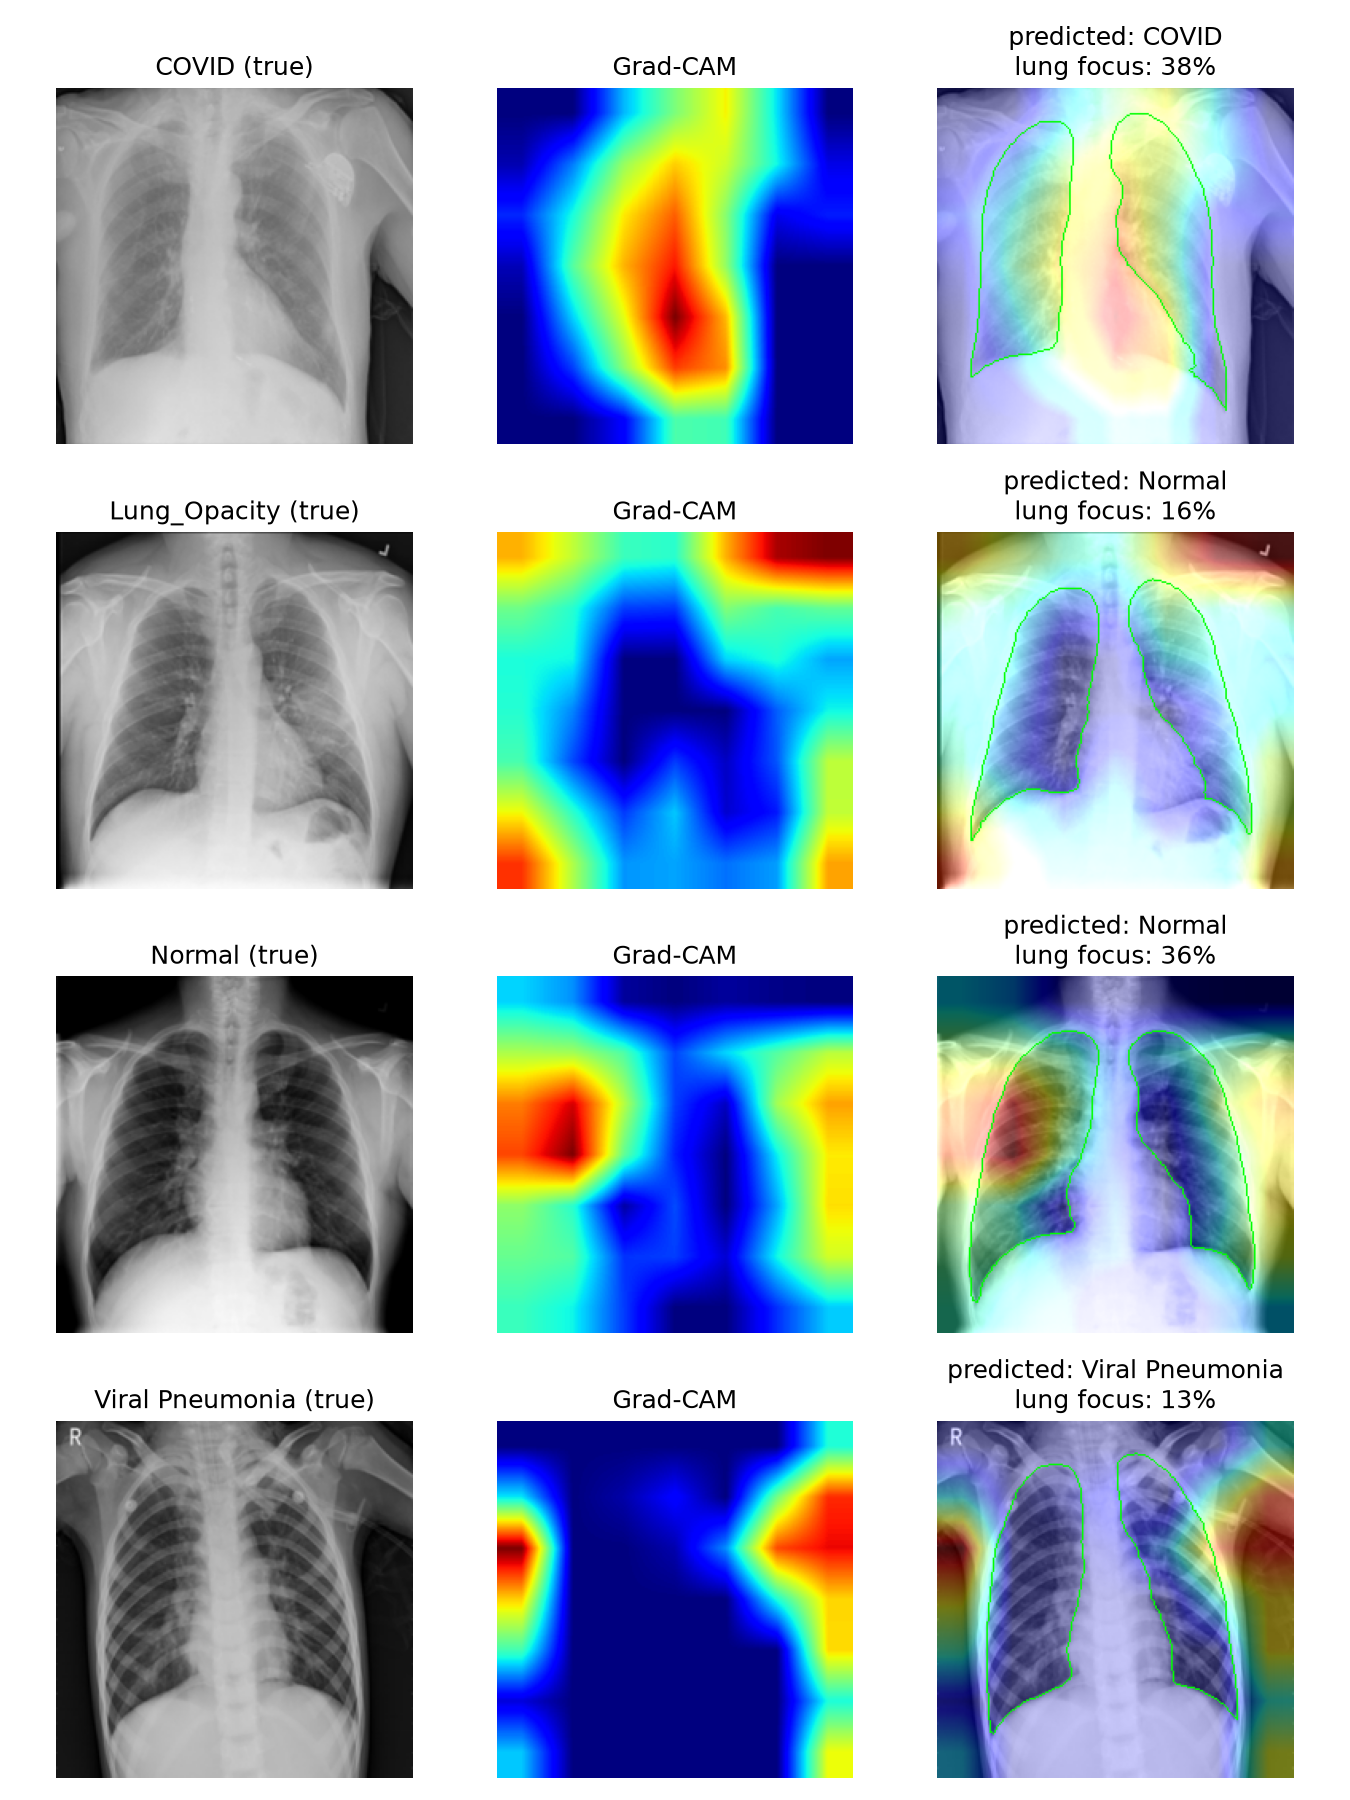
\includegraphics[width=0.9\linewidth]{figures/gradcam_transfer_baseline.png}
    \caption{Representative Grad-CAM examples for the frozen transfer model,
    with the lung mask boundary overlaid in green.}
    \label{fig:transfer_gradcam_baseline}
\end{figure}

Table~\ref{tab:transfer_lung_focus_baseline} quantifies this over 300
sampled test images.

\begin{table}[H]
\centering
\caption{Grad-CAM lung focus versus chance for the frozen transfer model.}
\label{tab:transfer_lung_focus_baseline}
\begin{tabular}{lccc}
\toprule
\textbf{Class} & \textbf{Grad-CAM in Lungs} & \textbf{Chance Level} & \textbf{Difference} \\
\midrule
COVID            & 30.8\% & 24.7\% & $+$6.1 pts \\
Normal           & 28.5\% & 25.0\% & $+$3.5 pts \\
Viral Pneumonia  & 29.8\% & 25.7\% & $+$4.2 pts \\
Lung Opacity     & 17.7\% & 20.6\% & $-$2.9 pts \\
\bottomrule
\end{tabular}
\end{table}

\begin{figure}[H]
    \centering
    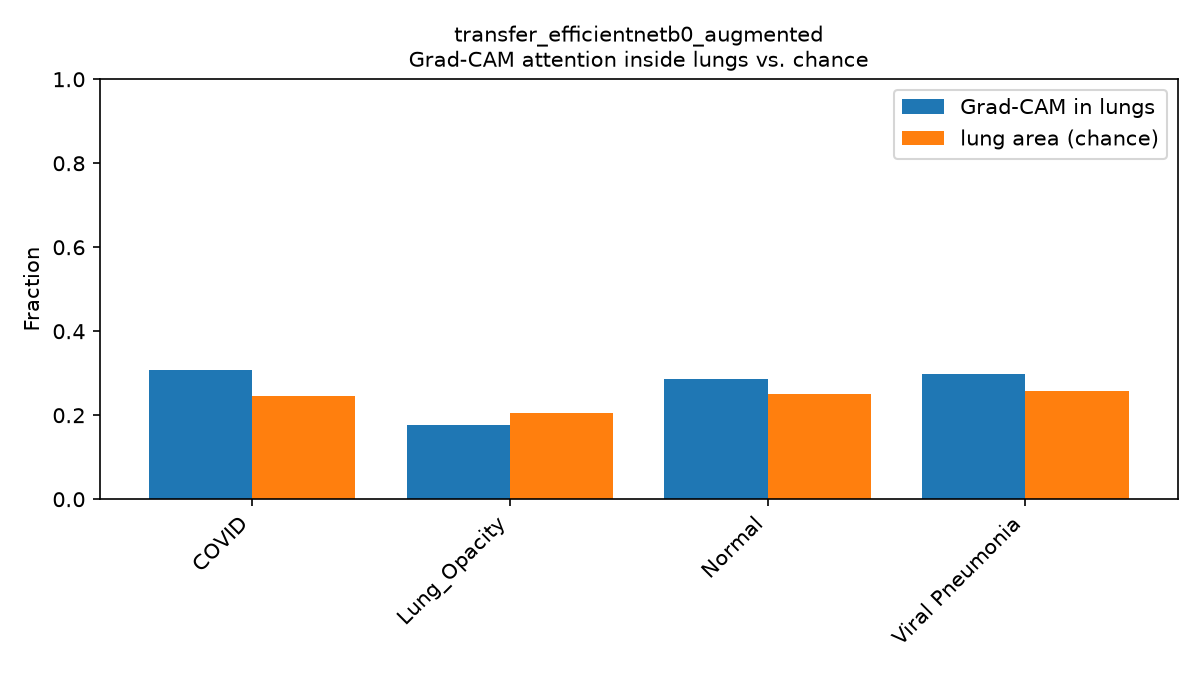
\includegraphics[width=0.7\linewidth]{figures/transfer_lung_focus_baseline.png}
    \caption{Grad-CAM attention inside the lungs versus the chance level, by
    class, for the frozen transfer model.}
    \label{fig:transfer_lung_focus_baseline}
\end{figure}

Attention is only mildly above chance for three of the four classes and
below chance for Lung Opacity, meaning the model attends to non-lung regions
more than pure geometry would predict for that class. Splitting the same
sample by prediction outcome showed virtually identical lung focus for
correct predictions (25.4\% versus a chance level of 23.7\%) and
misclassified predictions (25.2\% versus 22.5\%), indicating that weak
lung-focused attention is a systemic property of this model rather than an
error-specific artefact.

\subsection{Causal Test: Masking the Input}
\label{subsec:transfer_masking_causal}

Correlational Grad-CAM evidence cannot by itself establish that the model's
accuracy depends on non-pulmonary cues. A direct causal test was therefore
performed by training an otherwise identical model on images with every
pixel outside the lung mask forcibly set to zero before reaching the
network, so that no background information was available at all.

Table~\ref{tab:transfer_masked_causal} compares this masked model against
the frozen baseline.

\begin{table}[H]
\centering
\caption{Effect of masking the background at the input (causal test), test split.}
\label{tab:transfer_masked_causal}
\begin{tabular}{lccc}
\toprule
\textbf{Metric} & \textbf{Full Image} & \textbf{Lungs Only (Masked)} & \textbf{Change} \\
\midrule
Test accuracy      & 89.70\% & 83.07\% & $-$6.6 pts \\
Test macro F1       & 0.907   & 0.823   & $-$8.4 pts \\
COVID recall        & 90.3\%  & \textbf{57.0\%} & $-$33.3 pts \\
COVID F1            & 0.923   & 0.678   & $-$24.5 pts \\
Lung Opacity F1     & 0.854   & 0.809   & $-$4.5 pts \\
Normal F1           & 0.906   & 0.872   & $-$3.4 pts \\
Viral Pneumonia F1  & 0.945   & 0.932   & $-$1.3 pts \\
\bottomrule
\end{tabular}
\end{table}

If the model's accuracy depended evenly on pulmonary pathology, removing the
background should have degraded every class by a comparable amount.
Instead, the loss is heavily concentrated in COVID: recall collapses from
90.3\% to 57.0\%, a 33.3-point drop, meaning the masked model misses more
than 40\% of COVID cases that the full-image model correctly identified. The
other three classes lose only a few points each. This pattern is direct
causal evidence of COVID-specific background leakage in this dataset,
consistent with the widely reported concern that COVID images in this
Kaggle collection were aggregated from different sources than the other
classes, introducing incidental correlations unrelated to disease status.

As expected, Grad-CAM attention moves substantially into the lungs once the
background is physically removed, since no other information remains
available to the network (Table~\ref{tab:transfer_lung_focus_masked},
Figure~\ref{fig:transfer_gradcam_masked}).

\begin{table}[H]
\centering
\caption{Grad-CAM lung focus versus chance for the masked transfer model.}
\label{tab:transfer_lung_focus_masked}
\begin{tabular}{lccc}
\toprule
\textbf{Class} & \textbf{Grad-CAM in Lungs} & \textbf{Chance Level} & \textbf{Difference} \\
\midrule
COVID            & 40.8\% & 24.7\% & $+$16.1 pts \\
Lung Opacity     & 30.2\% & 20.6\% & $+$9.6 pts \\
Normal           & 49.4\% & 25.0\% & $+$24.4 pts \\
Viral Pneumonia  & 44.4\% & 25.7\% & $+$18.7 pts \\
\bottomrule
\end{tabular}
\end{table}

\begin{figure}[H]
    \centering
    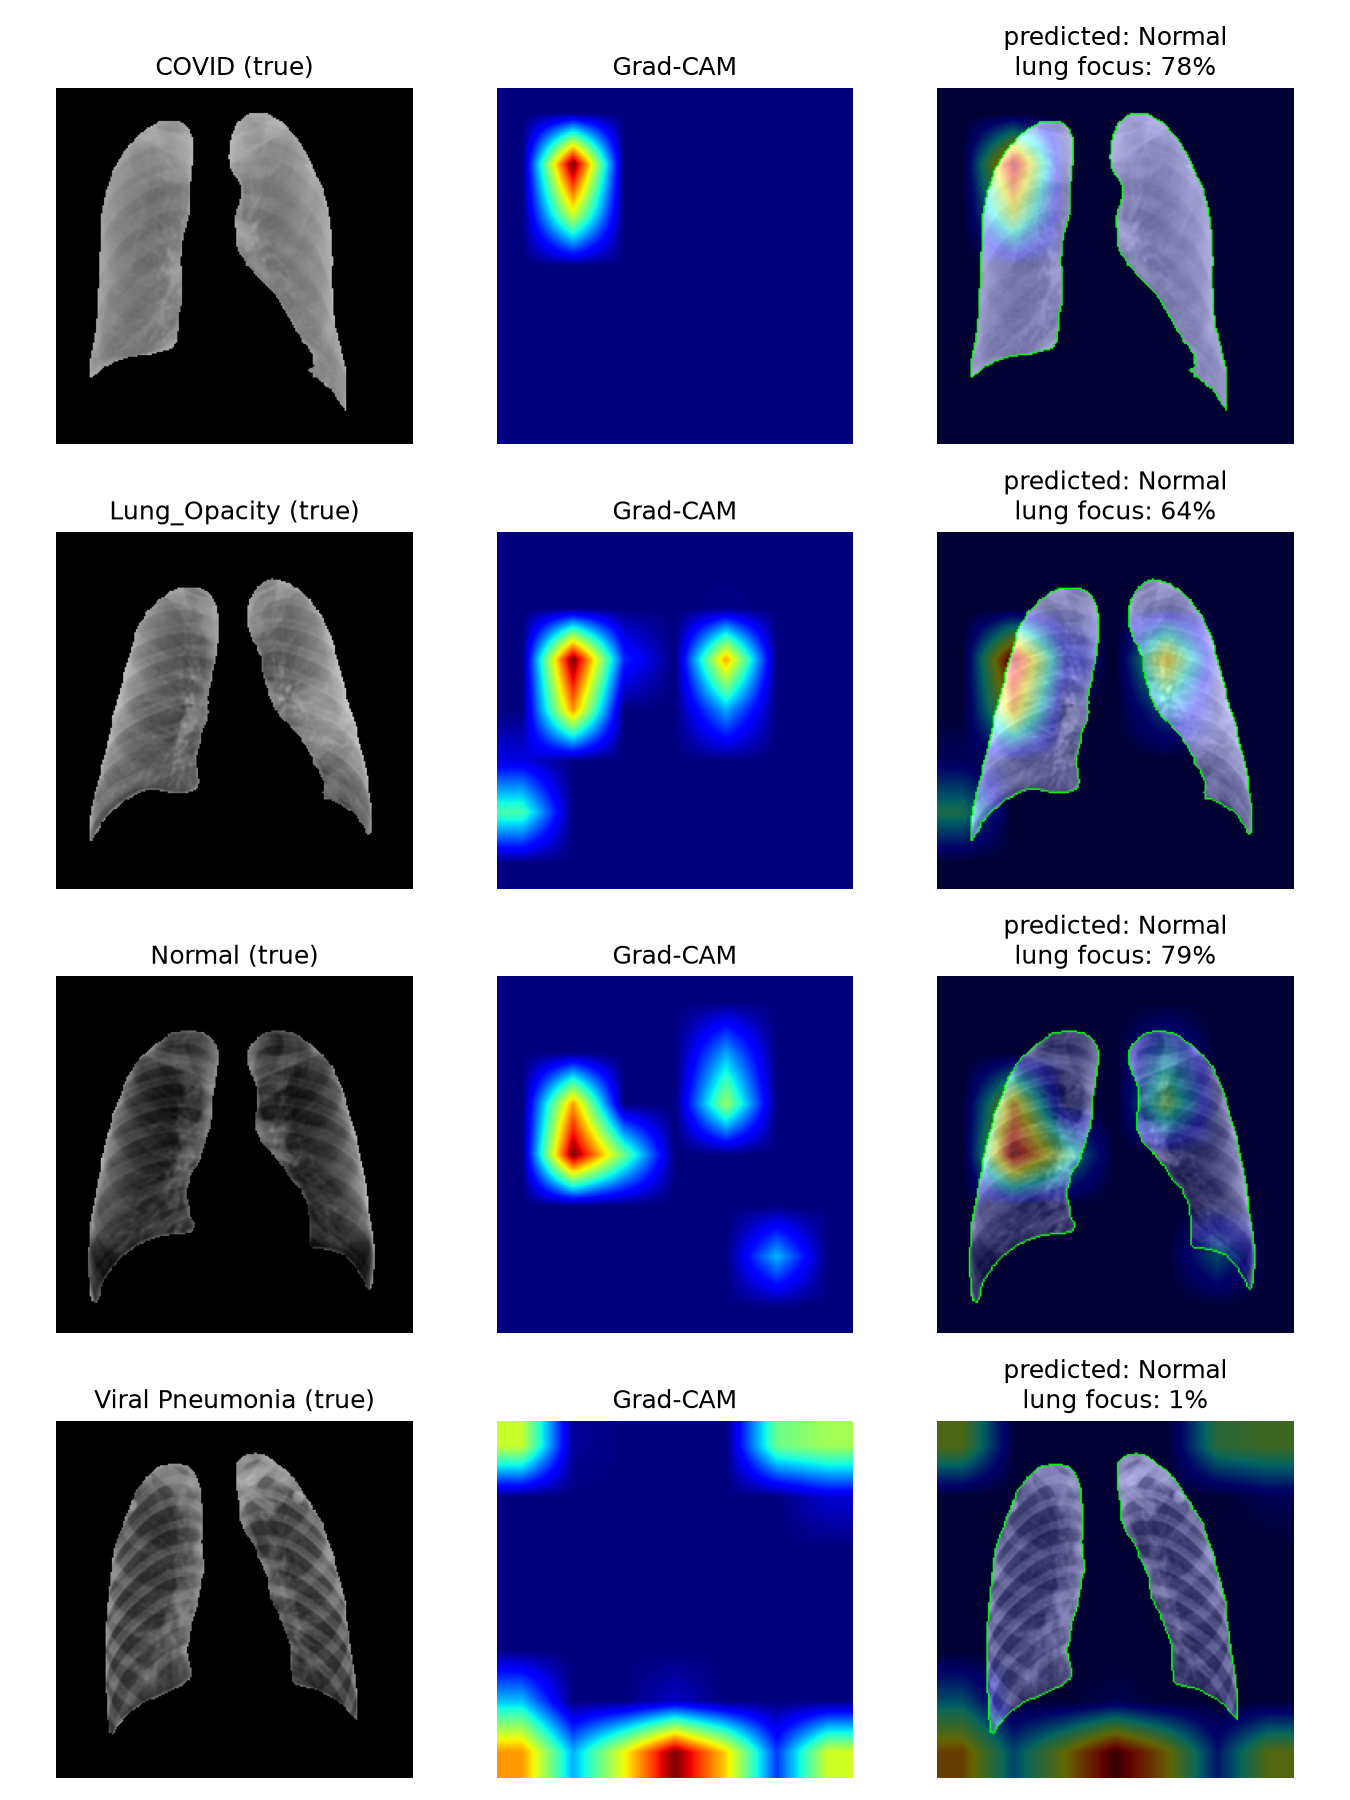
\includegraphics[width=0.9\linewidth]{figures/gradcam_transfer_masked.png}
    \caption{Representative Grad-CAM examples for the masked transfer model,
    with the lung mask boundary overlaid in green. All model input outside
    the boundary was zeroed before training and inference.}
    \label{fig:transfer_gradcam_masked}
\end{figure}

A small number of heatmap regions still extend outside the lung boundary
even though the corresponding input pixels were exactly zero. This is not
evidence that the masking failed; it is a known limitation of Grad-CAM on
deep convolutional networks, caused by non-zero learned biases and batch
normalisation statistics propagating through many stacked layers, together
with the coarse spatial resolution of the final convolutional feature map
and its associated large receptive field. For this reason, the aggregated
lung-focus statistics, and above all the masked-training accuracy
experiment itself, are treated as the primary evidence, rather than any
single Grad-CAM pixel.

\subsection{Isolating Shape: A Mask-Only Model}
\label{subsec:transfer_mask_only}

The masked model in Section~\ref{subsec:transfer_masking_causal} still
receives the lung's pixel intensities, that is, its texture and density
patterns, and only removes the background. To isolate lung \emph{shape}
from lung \emph{texture}, a further model was trained on the segmentation
masks themselves, that is, a binary lung silhouette with no pixel-intensity
information from the original radiograph at all.

Table~\ref{tab:transfer_mask_only} extends the comparison to this
shape-only model.

\begin{table}[H]
\centering
\caption{Decomposing accuracy into background, texture, and shape contributions (test split).}
\label{tab:transfer_mask_only}
\begin{tabular}{lccc}
\toprule
\textbf{Metric} & \textbf{Full Image} & \textbf{Lungs, Texture Kept} & \textbf{Shape Only} \\
\midrule
Test accuracy     & 89.70\% & 83.07\% & \textbf{74.07\%} \\
Test macro F1      & 0.907   & 0.823   & \textbf{0.703} \\
COVID recall       & 90.3\%  & 57.0\%  & \textbf{29.3\%} \\
COVID F1           & 0.923   & 0.678   & 0.413 \\
Normal F1          & 0.906   & 0.872   & 0.818 \\
Lung Opacity F1    & 0.854   & 0.809   & 0.709 \\
Viral Pneumonia F1 & 0.945   & 0.932   & 0.873 \\
\bottomrule
\end{tabular}
\end{table}

Lung shape alone is a weak classifier for COVID, with recall of 29.3\%,
close to what a random four-class guess would achieve, while Normal cases
remain comparatively easier to recognise from shape alone (F1 0.818). The
test confusion matrix (Figure~\ref{fig:transfer_mask_only_confusion}) shows
that, of the true COVID cases, the shape-only model most often mistakes them
for Normal or Lung Opacity, consistent with COVID's radiographic signature
being primarily about tissue density and opacity patterns inside the lung
field rather than its outline.

\begin{figure}[H]
    \centering
    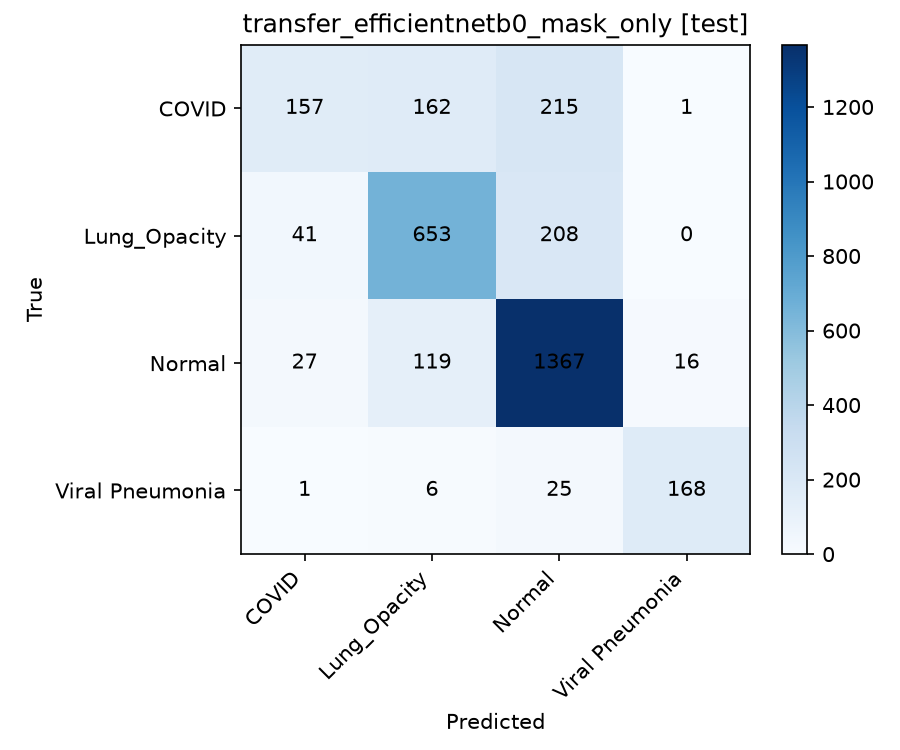
\includegraphics[width=0.55\linewidth]{figures/transfer_mask_only_confusion.png}
    \caption{Test-set confusion matrix for the shape-only (mask-only) transfer model.}
    \label{fig:transfer_mask_only_confusion}
\end{figure}

Taken together, Sections~\ref{subsec:transfer_masking_causal} and
\ref{subsec:transfer_mask_only} give a three-way decomposition of the frozen
model's 89.70\% test accuracy: approximately 6.6 points depend on non-lung
background and context, a further approximately 9.0 points depend on lung
texture and density patterns rather than shape, and the remainder is what
lung geometry alone can achieve, well above the 25\% random baseline but a
weak classifier by itself, and specifically unreliable for COVID.

\subsection{An Architectural Alternative: Masked Pooling}
\label{subsec:transfer_masked_pooling}

Hard input masking (Section~\ref{subsec:transfer_masking_causal}) is an
effective causal probe, but it discards all information outside the lungs
even where that information might legitimately help, for example by
providing context for image quality or overall framing, and it costs
several points of raw performance. As a softer alternative, a masked global
average pooling layer was used instead: rather than zeroing the input image,
the model's final convolutional feature map is masked so that only
lung-covering spatial locations contribute to the pooled features that feed
the classification head, while the backbone still observes the full image.

This configuration, combined with class balancing and rotation-only
augmentation, reached \textbf{88.79\%} test accuracy and \textbf{0.897}
macro F1, recovering to within roughly one accuracy point of the frozen
full-image baseline while still architecturally constraining the features
used for classification to the lung region. This suggests that how a model
is restricted to the lungs, that is, at the input versus within the pooling
operation, materially affects the performance cost of enforcing that
constraint, and is a useful direction for future work aiming to reduce
background reliance without the full accuracy cost of hard input masking.

\subsection{Grad-CAM on the Fine-Tuned Model}
\label{subsec:transfer_gradcam_finetuned}

The same lung-focus analysis was repeated for the fine-tuned model of
Section~\ref{sec:transfer_finetune}, the best-performing model in this
project. Table~\ref{tab:transfer_lung_focus_finetuned} reports the
per-class results.

\begin{table}[H]
\centering
\caption{Grad-CAM lung focus versus chance for the fine-tuned transfer model.}
\label{tab:transfer_lung_focus_finetuned}
\begin{tabular}{lccc}
\toprule
\textbf{Class} & \textbf{Grad-CAM in Lungs} & \textbf{Chance Level} & \textbf{Difference} \\
\midrule
COVID            & 24.3\% & 24.4\% & $-$0.1 pts \\
Lung Opacity     & 31.2\% & 20.9\% & $+$10.3 pts \\
Normal           & 38.5\% & 25.2\% & $+$13.3 pts \\
Viral Pneumonia  & 23.8\% & 24.0\% & $-$0.2 pts \\
\bottomrule
\end{tabular}
\end{table}

Fine-tuning changes which classes show above-chance lung attention: Lung
Opacity and Normal now show clearly above-chance attention, the opposite of
the frozen baseline's pattern in
Table~\ref{tab:transfer_lung_focus_baseline}, while COVID and Viral
Pneumonia sit almost exactly at chance. This differs from the CNN-from-
scratch full-image baseline's attention pattern
(Section~\ref{subsec:full_gradcam}), where COVID and Normal were close to
proportional and Lung Opacity was the weakest. The two architectures
therefore appear to rely on different, model-specific combinations of
pulmonary and non-pulmonary cues, even though both ultimately fall short of
attention that is consistently and exclusively pulmonary. Given the masking
experiments in Section~\ref{subsec:transfer_masking_causal}, the near-chance
COVID attention of the fine-tuned model is a reminder that its very high
COVID recall (97.8\%, Table~\ref{tab:transfer_finetuned_results}) should not
be assumed to reflect improved pulmonary diagnosis without further,
dedicated causal testing on this specific model.

\section{Comparison with the CNN-from-Scratch Baselines and Conclusions}
\label{sec:transfer_comparison}

Table~\ref{tab:transfer_full_comparison} brings together the CNN-from-scratch
baselines of Section~\ref{sec:baselines} and the transfer-learning models of
this chapter on the common test split.

\begin{table}[H]
\centering
\caption{Comparison of all principal models evaluated in this project (test split).}
\label{tab:transfer_full_comparison}
\begin{tabular}{lcc}
\toprule
\textbf{Model} & \textbf{Test Accuracy} & \textbf{Macro F1} \\
\midrule
Simple CNN, full image        & 81.96\% & 0.827 \\
Simple CNN, lung-ROI          & 78.71\% & 0.774 \\
Transfer, frozen EfficientNetB0 & 89.70\% & 0.907 \\
Transfer, augmented (no flip) & 88.38\% & 0.896 \\
Transfer, fine-tuned          & \textbf{92.36\%} & \textbf{0.936} \\
\bottomrule
\end{tabular}
\end{table}

Figure~\ref{fig:transfer_all_runs_comparison} shows the same comparison
extended to every transfer-learning run trained in this chapter.

\begin{figure}[H]
    \centering
    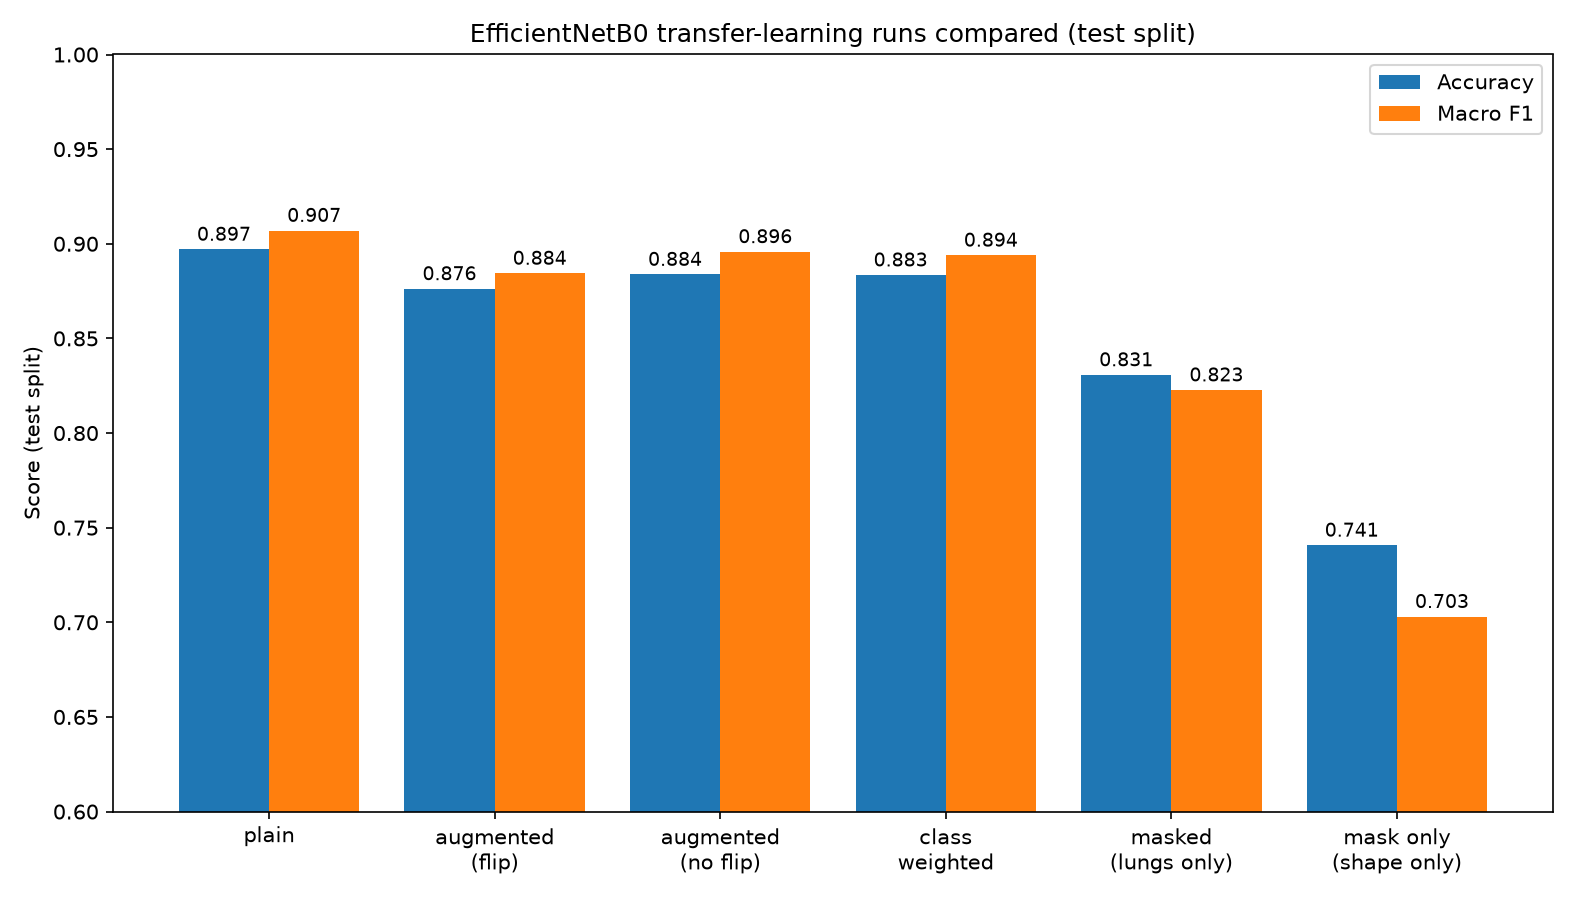
\includegraphics[width=0.95\linewidth]{figures/transfer_all_runs_comparison.png}
    \caption{Test accuracy and macro F1 across all EfficientNetB0
    transfer-learning runs compared in this chapter.}
    \label{fig:transfer_all_runs_comparison}
\end{figure}

Three conclusions follow from this chapter, in line with the project's
Step 3 objective of drawing scientific and business conclusions from the
success or failure of the modelling phase.

First, transfer learning substantially outperforms training a comparable
CNN from scratch on this dataset, and fine-tuning the backbone end-to-end
gives the strongest result obtained anywhere in this project (92.36\%
accuracy, 0.936 macro F1). This is consistent with the dataset being too
small, relative to the visual complexity of chest radiographs, for a
from-scratch model to learn as effective a feature representation as one
pretrained on a much larger, general-purpose image corpus.

Second, this headline performance is not fully attributable to pulmonary
pathology. The interpretability analysis in
Section~\ref{sec:transfer_interpretability} shows that a meaningful share of
the frozen model's accuracy, and specifically its COVID recall, depends on
non-anatomical cues in this Kaggle dataset rather than lung tissue itself.
The fine-tuned model's near-chance COVID attention
(Section~\ref{subsec:transfer_gradcam_finetuned}) suggests this concern is
not resolved simply by improving raw accuracy through fine-tuning, and may
require dedicated causal testing analogous to
Section~\ref{subsec:transfer_masking_causal} before it can be ruled out.

Third, and consequently, the headline accuracy of the best model in this
project should not be read as evidence of clinical readiness. As with the
CNN-from-scratch baselines, this remains an educational decision-support
study rather than a validated diagnostic system, and any future external
validation of this model line should specifically test for COVID-recall
collapse on radiographs from sources not represented in this training
dataset, since that is precisely the failure mode predicted by the
background-leakage evidence in this chapter.
